\documentclass{article}
\usepackage{tikz}

\begin{document}

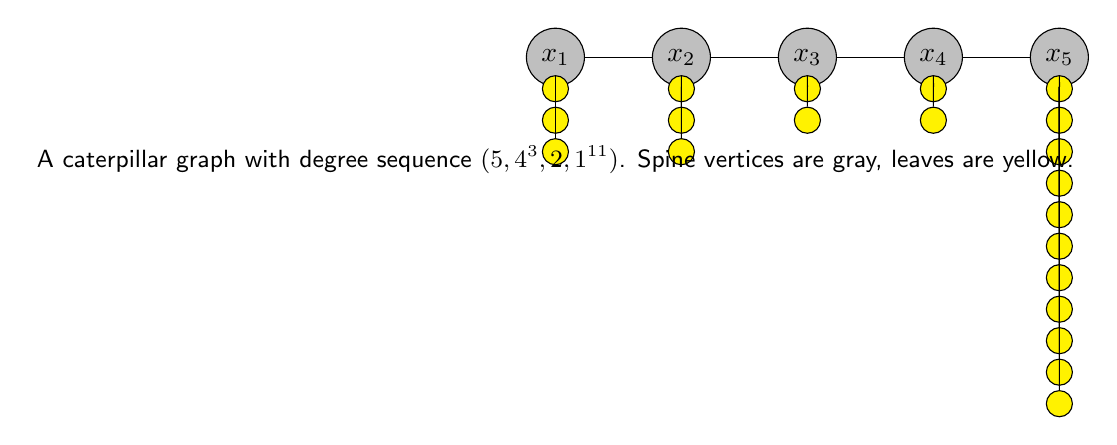
\begin{tikzpicture}[scale=0.8]
    % Define the positions of the nodes
    \node[circle,fill=gray!50,draw] (x1) at (0,0) {$x_1$};
    \node[circle,fill=gray!50,draw] (x2) at (2,0) {$x_2$};
    \node[circle,fill=gray!50,draw] (x3) at (4,0) {$x_3$};
    \node[circle,fill=gray!50,draw] (x4) at (6,0) {$x_4$};
    \node[circle,fill=gray!50,draw] (x5) at (8,0) {$x_5$};

    % Draw the edges between the spine nodes
    \draw (x1) -- (x2);
    \draw (x2) -- (x3);
    \draw (x3) -- (x4);
    \draw (x4) -- (x5);

    % Draw the leaves connected to each spine node
    \foreach \i in {1,...,3} {
        \node[circle,fill=yellow,draw] (y\i) at (0,-0.5*\i) {};
        \draw (x1) -- (y\i);
    }
    \foreach \i in {1,...,3} {
        \node[circle,fill=yellow,draw] (y\i) at (2,-0.5*\i) {};
        \draw (x2) -- (y\i);
    }
    \foreach \i in {1,...,2} {
        \node[circle,fill=yellow,draw] (y\i) at (4,-0.5*\i) {};
        \draw (x3) -- (y\i);
    }
    \foreach \i in {1,...,2} {
        \node[circle,fill=yellow,draw] (y\i) at (6,-0.5*\i) {};
        \draw (x4) -- (y\i);
    }
    \foreach \i in {1,...,11} {
        \node[circle,fill=yellow,draw] (y\i) at (8,-0.5*\i) {};
        \draw (x5) -- (y\i);
    }

    % Caption
    \node[below=1cm] {\small\sf A caterpillar graph with degree sequence $(5,4^3,2,1^{11})$. Spine vertices are gray, leaves are yellow.};
\end{tikzpicture}

\end{document}